\documentclass[aspectratio=169,11pt]{beamer}

\usepackage{svg}
\usepackage{tikz}
\usetheme{Boadilla}
\definecolor{gxsmblue}{HTML}{105C78}
\definecolor{gxsmcyan}{HTML}{00ADDC}
\definecolor{gxsmlime}{HTML}{B2D33B}
\definecolor{gxsmhighlight}{HTML}{F4D985}
\definecolor{gxsmhighlightbody}{HTML}{FFF8E5}
\setbeamercolor{structure}{fg=gxsmblue}
\setbeamercolor{frametitle}{fg=white,bg=gxsmblue}
\setbeamercolor{title}{fg=white}
\setbeamercolor{block title}{fg=black,bg=gxsmhighlight}
\setbeamercolor{block body}{fg=black,bg=gxsmhighlightbody}
\setbeamercolor{block title alerted}{fg=black,bg=gxsmhighlight}
\setbeamercolor{block body alerted}{fg=black,bg=gxsmhighlightbody}
\setbeamertemplate{navigation symbols}{}
\setbeamertemplate{footline}[frame number]
\setbeamertemplate{itemize item}{\color{gxsmblue}\small$\blacktriangleright$}
\setbeamertemplate{itemize subitem}{\color{gxsmlime!70!black}\tiny$\bullet$}
\usebackgroundtemplate{%
  
\includegraphics[width=\paperwidth,height=\paperheight]{backgrounds/content-background.jpeg}}

\begin{document}

{\usebackgroundtemplate{%
  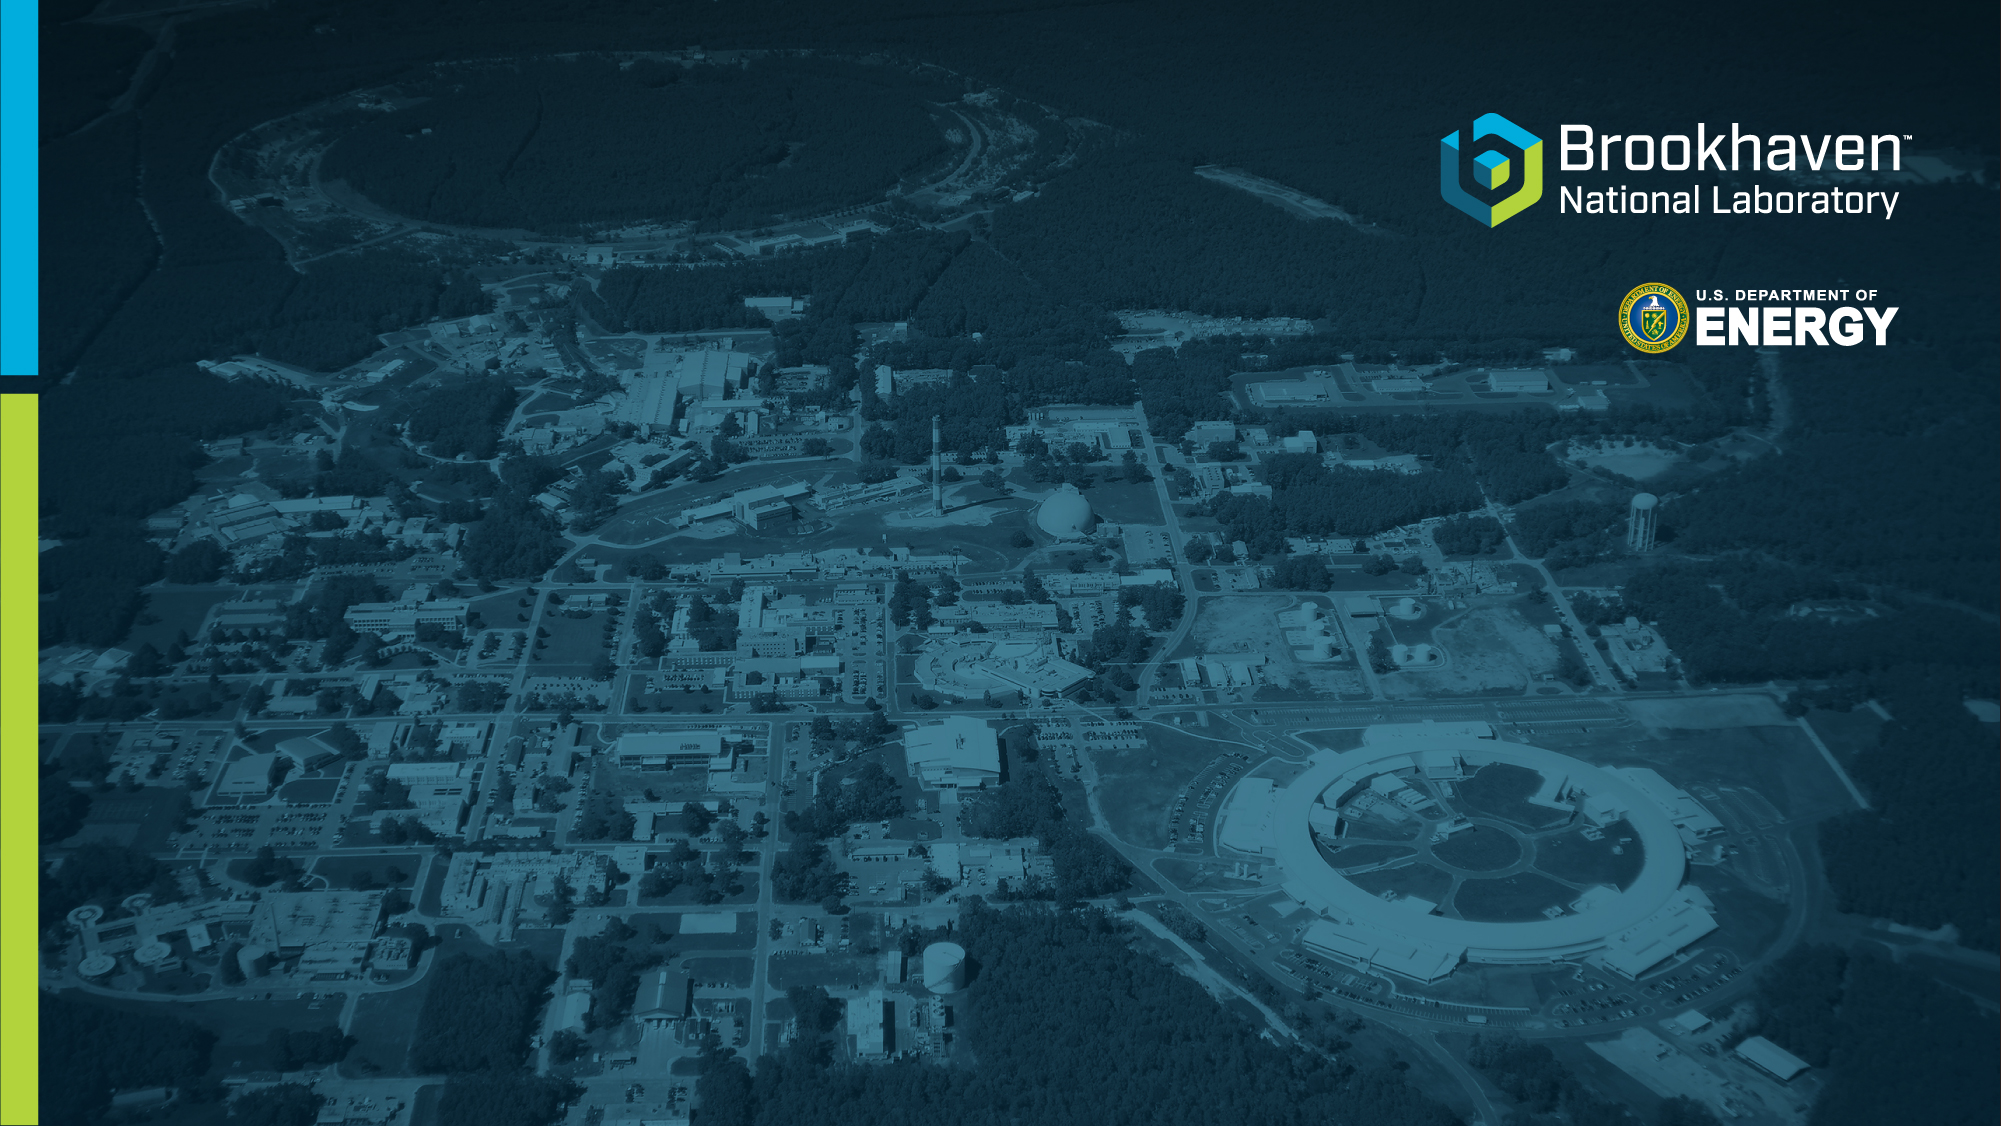
\includegraphics[width=\paperwidth,height=\paperheight]{backgrounds/dark-background.jpeg}}
\begin{frame}[plain]
  \color{white}
  \centering
  \vspace{0.55cm}
  \begin{minipage}{0.78\textwidth}
    \raggedright
    \includesvg[width=0.12\textwidth,inkscapelatex=false]{../../../icons/gxsm4-icon}
    \par\vspace{0.18cm}
    {\Huge\bfseries GXSM4\par}
    \vspace{0.06cm}
    {\LARGE\bfseries Local Microscope Copilot\par}
    \vspace{0.12cm}
    {\large Percy Zahl --- Staff Scientist, CFN\par}
    \vspace{0.38cm}
    \small
    This project adds a local AI copilot to GXSM4 scanning probe microscopy:
    combining live readbacks, scan and tip analysis, and carefully gated
    assistance. You will use AI tools to accelerate development and build an
    SPM-focused agent for complex tasks, while creating features, tests, and
    verification workflows for supervised instrument use.
  \end{minipage}
\end{frame}
}

\begin{frame}{Local Microscope Copilot}
  \centering
  \large\textit{The project and what you will build}
  \par\vspace{0.6em}
  \small
  \begin{columns}[T,onlytextwidth]
    \column{0.48\textwidth}
      \textbf{The idea}
      \begin{itemize}
        \item Make repetitive microscope work easier to inspect and carry out.
        \item Combine a local Python controller and GUI with AI-assisted interpretation and analysis.
        \item Keep the operator in control: monitoring and analysis are distinct from hardware-changing actions.
      \end{itemize}
    \column{0.48\textwidth}
      \textbf{What is already here}
      \begin{itemize}
        \item Live readbacks, scan views, and tip/landscape analysis.
        \item Explicitly gated scan controls and GVP tip-tuning workflows.
        \item Safety levels, dry-run operation, confirmations, and action history.
      \end{itemize}
  \end{columns}
\end{frame}

\begin{frame}{Your project across the full stack}
  \footnotesize
  \begin{columns}[T,onlytextwidth]
    \column{0.49\textwidth}
      \textbf{Understand the system}
      \begin{itemize}
        \setlength{\itemsep}{0pt}\setlength{\topsep}{0pt}
          \item You will explore the GUI, controller, GXSM4 interface, and configuration.
          \item You will learn microscope signals, coordinates, units, and operating limits.
      \end{itemize}
      \textbf{Test and verify}
      \begin{itemize}
        \setlength{\itemsep}{0pt}\setlength{\topsep}{0pt}
        \item You will build tests for conversions, safety limits, and AI-generated proposals.
        \item You will verify GUI/controller behavior, dry-runs, blocked actions, and recovery.
      \end{itemize}
    \column{0.49\textwidth}
      \textbf{Create and improve}
      \begin{itemize}
        \setlength{\itemsep}{0pt}\setlength{\topsep}{0pt}
        \item You will extend scan/tip analysis and the tip-tuning planner.
        \item You will prototype an SPM agent that proposes steps, expected readbacks, and stop conditions.
        \item You will measure reliability and responsiveness, then improve usability and diagnostics.
      \end{itemize}
  \end{columns}
  \vspace{0.1em}
  \begin{block}{Hands-on with staff experts}
    \footnotesize
    You will work with instrument experts on a top-tier low-temperature ($\sim$4 K)
    LT-STM/AFM with high-resolution AFM (HR-AFM)—connecting software and tests
    directly to experiments.
  \end{block}
\end{frame}

\begin{frame}{From tests to reliable real-world use}
  \footnotesize
  \setlength{\itemsep}{0.2em}
  \begin{enumerate}
    \item \textbf{Offline first} — you will test coordinate conversions, configuration, and safety limits with known inputs.
    \item \textbf{Dry-run next} — you will check proposed actions, confirmations, cancellation, and failure cases without hardware changes.
    \item \textbf{Verify integration} — you will test GUI/controller paths and GXSM4 reads; compare readbacks in a safe test setup.
    \item \textbf{Supervised trials} — you will follow an operator-approved protocol, begin read-only, then verify each bounded live action.
  \end{enumerate}
  \vspace{0.2em}
  \begin{block}{A successful project outcome}
    A repeatable, tested workflow with clear limits and documented verification.
  \end{block}
  \begin{alertblock}{Safety boundary}
    No unattended hardware control. Live trials require operator approval and direct supervision.
  \end{alertblock}
\end{frame}

{\usebackgroundtemplate{%
  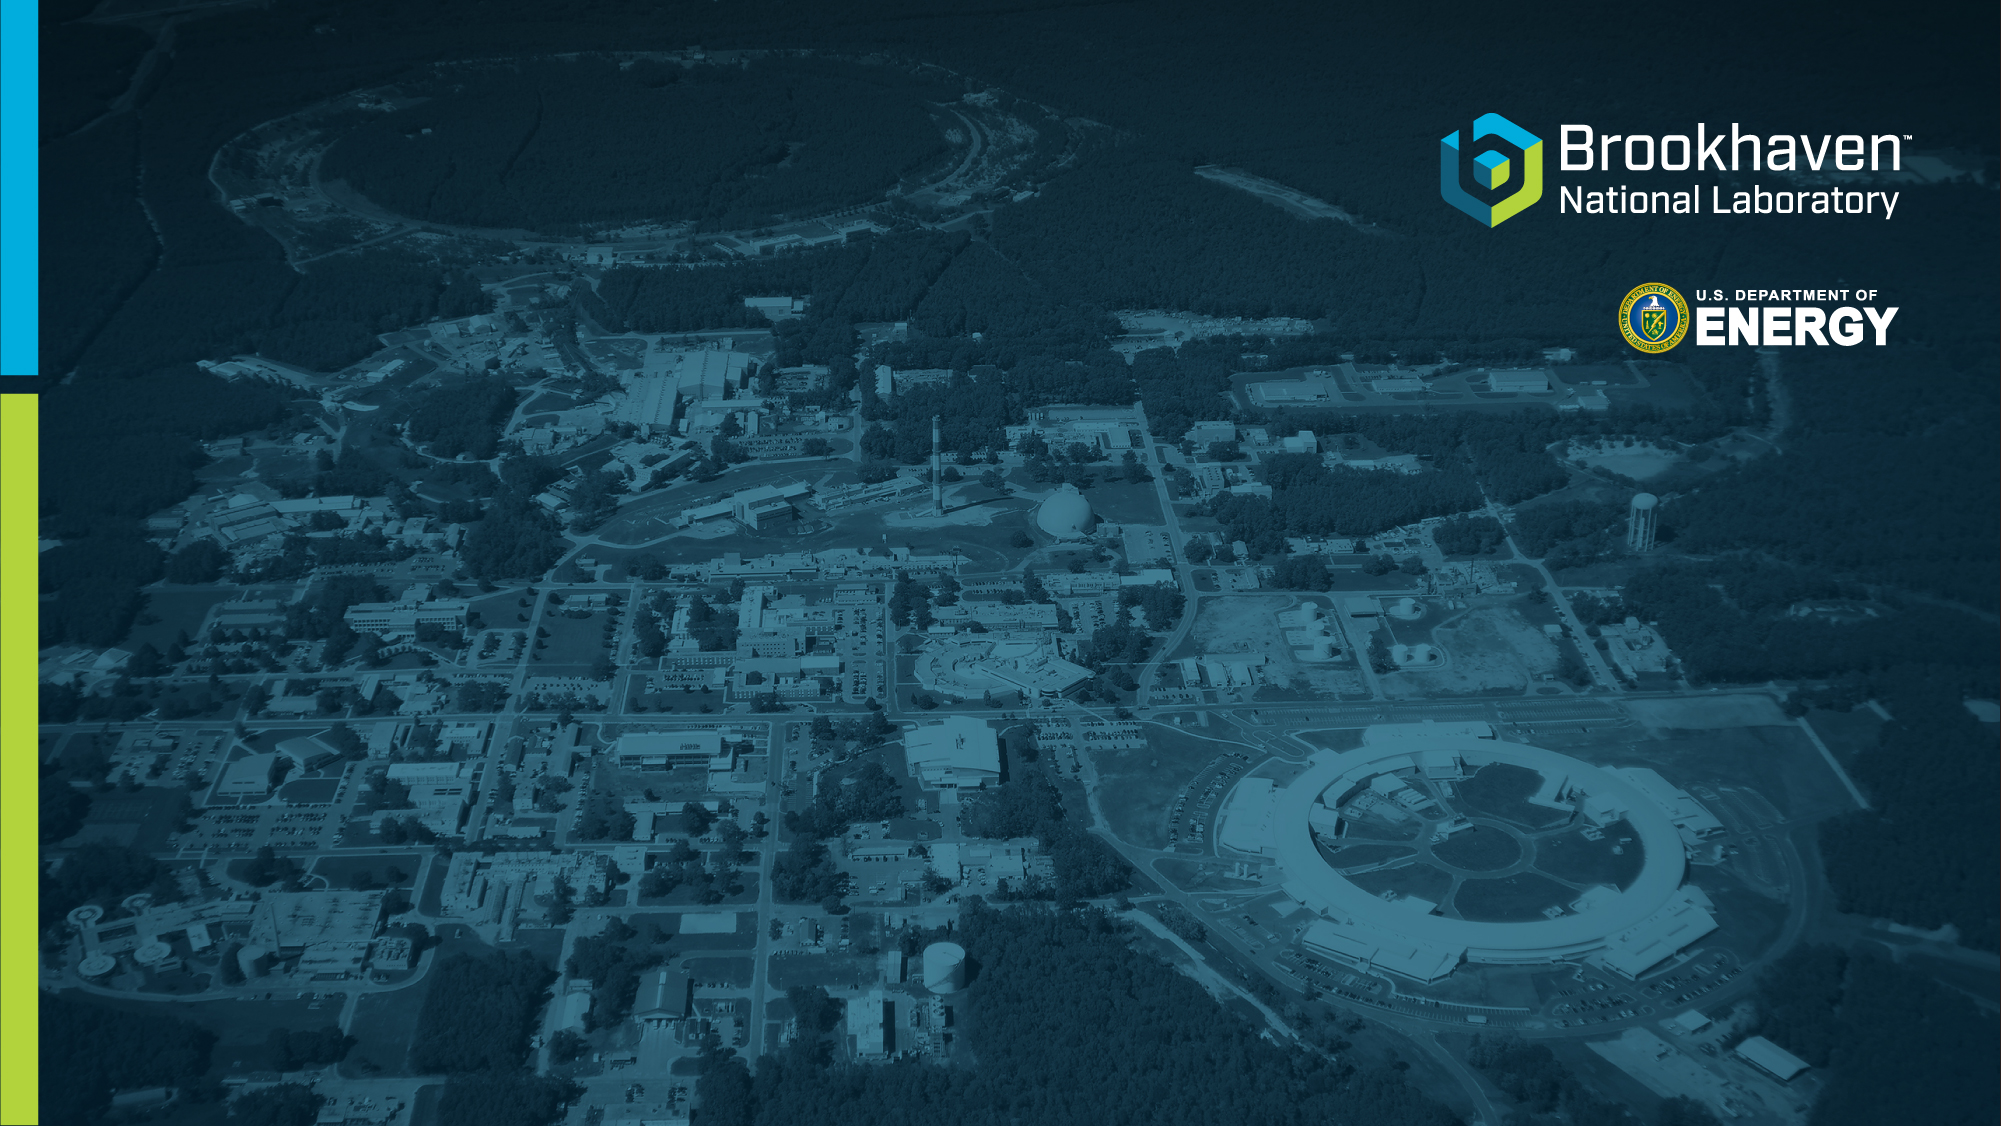
\includegraphics[width=\paperwidth,height=\paperheight]{backgrounds/dark-background.jpeg}}
\setbeamercolor{normal text}{fg=white}
\setbeamercolor{itemize/enumerate body}{fg=white}
\setbeamercolor{itemize item}{fg=white}
\setbeamertemplate{itemize item}{\color{white}\small$\blacktriangleright$}
\begin{frame}{Molecular structures revealed with HR-AFM}
  \usebeamercolor[fg]{normal text}
  \footnotesize
  \begin{columns}[T,onlytextwidth]
    \column{0.67\textwidth}
      \begin{tikzpicture}
        \node[anchor=south west,inner sep=0] (newsimage) {
          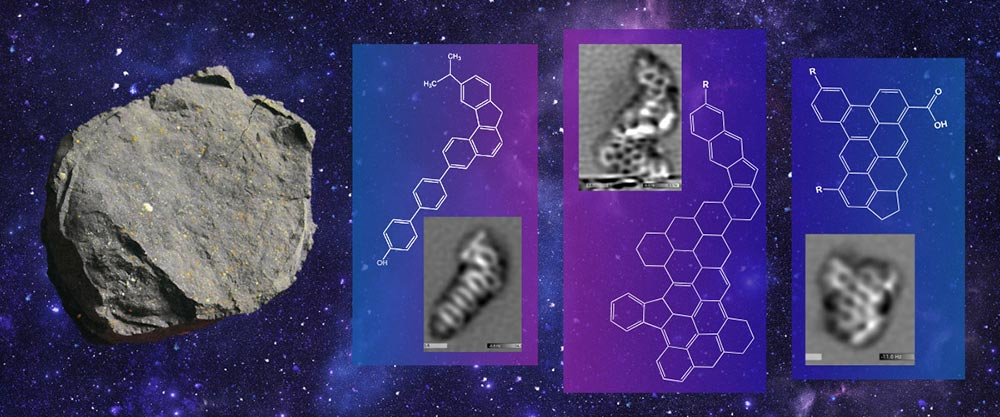
\includegraphics[width=\linewidth,height=0.47\textheight,keepaspectratio]{figures/meteorite-molecules.jpg}
        };
        \node[anchor=south west,fill=white,inner sep=2pt,rounded corners=1pt]
          at ([xshift=0.12cm,yshift=0.12cm]newsimage.south west) {
            
\includegraphics[height=1.15cm]{figures/bnl-story-qr.png}
          };
      \end{tikzpicture}
      \par\vspace{0.2em}
      \tiny
      \textcolor{white}{Image: Edan Schultz / National MagLab, via Brookhaven National Laboratory.
      \href{https://www.bnl.gov/newsroom/news.php?a=123172}{Read the BNL story}.}
    \column{0.30\textwidth}
      \vspace{1.9cm}
      \scriptsize
      \textbf{A real-world SPM achievement}
      \begin{itemize}
        \setlength{\itemsep}{0pt}\setlength{\topsep}{0pt}
        \item HR-nc-AFM revealed individual organic molecules in meteorite samples.
        \item Expert practice and careful image interpretation made this possible.
        \item The results offer a glimpse into our solar system's origins.
      \end{itemize}
  \end{columns}
  \vspace{-0.23cm}
  \begin{block}{Your challenge}
    \scriptsize
    You will build and verify an AI copilot to ease repetitive, complex SPM work, give experts more time for science, and make better use of instrument time---potentially 24/7.
  \end{block}
\end{frame}
}

\end{document}
